\documentclass{standalone}
%% Show/hide steps for standalone work — edit this line:
\makeatletter\AtBeginDocument{\@buildstepset{1,2}}\makeatother
\usepackage{tikz}
\usetikzlibrary{intersections,calc}
\usepackage{amsmath}
\usepackage{hsbcommon}
\begin{document}
    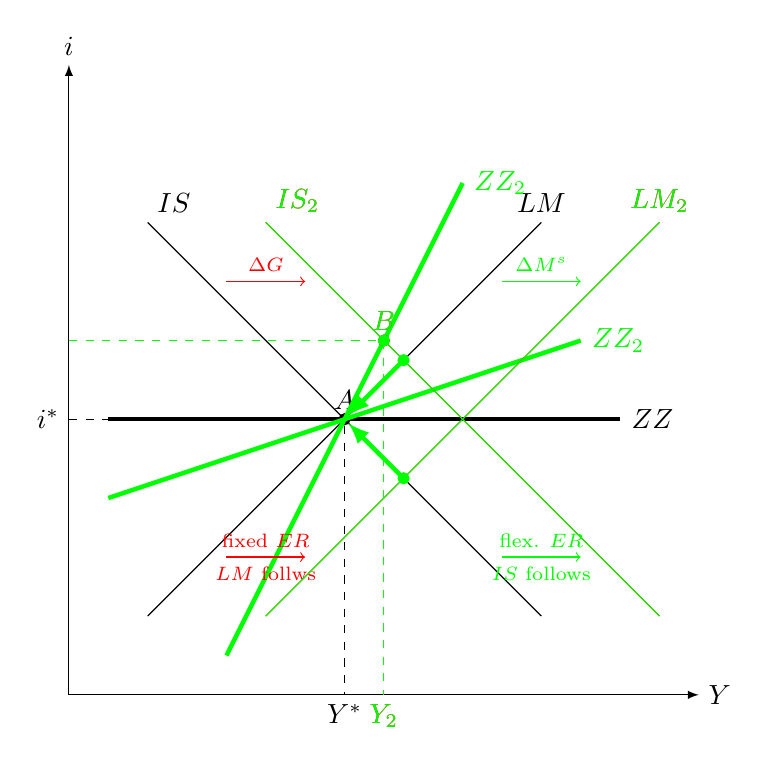
\begin{tikzpicture}
        \draw[->,>=latex] (0,0) -- (8,0) node (Y) [right] {$Y$};
        \draw[->,>=latex] (0,0) -- (0,8) node (i) [above] {$i$};

        \draw[name path=is] (1,6) node[above right] {$IS$} -- (6,1);
        \draw[name path=lm] (1,1) -- (6,6) node[above] {$LM$};

        \path [name intersections={of=is and lm, by=E}];
        \filldraw (E) circle (2pt) node[above] {$A$};
        \draw[dashed] (i |- E) node [left] {$i^*$} -- (E) -- (E |- Y) node [below] {$Y^*$};

        %% ZZ curve (world interest rate with perfect capital mobility, BoP balance curve)
            \draw[ultra thick, name path=zz] (0.5, |- E) -- (7, |- E) node [right] {$ZZ$};

        %% alternatively: ZZ curve with capital controls, 2 versions (less / more steep)
        \ifstep{10}{
            \draw[green,ultra thick, name path=zz] ($(E)+(-3,-1)$) -- ($(E)+(3,1)$) node [right] {$ZZ_2$};
        }
        \ifstep{11}{
            \draw[green,ultra thick, name path=zz] ($(E)+(-1.5,-3)$) -- ($(E)+(1.5,3)$) node [right] {$ZZ_2$};
        }

        %%%%%%%%%% Original IS-LM situation

        \begin{scope}[xshift=1.5cm]    
            \path[name path global=is2] (1,6)  -- (6,1);
            \path[name path global=lm2] (1,1) -- (6,6) ;
            \path [name intersections={of=is2 and lm,  by=F1}];
            \path [name intersections={of=is and lm2, by=F2}];            
            \path [name intersections={of=is2 and zz,  by=G1}];
        \end{scope}

        %% Step 1: IS curve shift first
        \ifstep{1}{
            \begin{scope}[color=red]
                \begin{scope}[xshift=1.5cm]
                    \draw  (1,6) node[above right] {$IS_2$} -- (6,1);
                    \draw[->] (0.5,5.25) -- node[above] {\scriptsize $\Delta G$} (1.5,5.25) ;
                \end{scope}
            \end{scope}
        }

        \ifsteponly{1}{2,3,4}{ %% snap back arrow
            \filldraw[green] (F1) circle (2pt) ;
            \draw[green,->,ultra thick,>=latex,shorten >=2pt] (F1) --  (E);
        }
        %% Step 2: IS curve shift, LM follows
        \ifstep{2}{
            \begin{scope}[color=red]
                \begin{scope}[xshift=1.5cm]
                    \draw (1,1) -- (6,6) node[above] {$LM_2$};
                    \filldraw (G1) circle (2pt) node[above] {$B$};
                    \draw[->] (0.5,1.75) -- node[above] {\scriptsize fixed $ER$} node[below] {\scriptsize $LM$ follws}(1.5,1.75) ;
                \end{scope}
                \draw[dashed] (i |- G1) -- (G1) -- (G1 |- Y) node [below] {$Y_2$};
            \end{scope}
        }
        
        %% Step 3: LM curve shift first
        \ifstep{3}{
            \begin{scope}[color=green]
                \begin{scope}[xshift=1.5cm]
                    \draw (1,1) -- (6,6) node[above] {$LM_2$};
                    \draw[->] (4,5.25) -- node[above] {\scriptsize  $\Delta M^s$ } (5,5.25) ;
                \end{scope}
            \end{scope}
        }
        \ifsteponly{3}{1,2,4}{ %% snap back arrow
            \draw[green,->,ultra thick,>=latex,shorten >=2pt] (F2) --  (E);
            \filldraw[green] (F2) circle (2pt) ;
        }
        %% Step 4: LM curve shift, IS follows
        \ifstep{4}{
            \begin{scope}[color=green]
                \begin{scope}[xshift=1.5cm]
                    \draw  (1,6) node[above right] {$IS_2$} -- (6,1);
                    % \filldraw (F1) circle (2pt) node[above] {$P$};
                    \draw[->] (4,1.75) -- node[above] {\scriptsize flex. $ER$} node[below] {\scriptsize $IS$ follows} (5,1.75) ;
                    \filldraw (G1) circle (2pt) node[above] {$B$};                    
                \end{scope}
                \draw[dashed] (i |- G1) -- (G1) -- (G1 |- Y) node [below] {$Y_2$};
            \end{scope}
        }
 

    \end{tikzpicture}
\end{document}